%% rnaastex.cls is the classfile used for Research Notes. It is derived
%% from aastex61.cls with a few tweaks to allow for the unique format required.
\documentclass[modern]{rnaastex}

\usepackage{graphicx}
\usepackage[suffix=]{epstopdf}
\usepackage{natbib}
\usepackage{amsmath}
\usepackage{xspace}
\usepackage{url}

\newcommand{\ingot}{{\tt ingot}\xspace} % floating space at the end is key!
%\newcommand{\feh}{$[\mathrm{M}/\mathrm{H}]$}
\newcommand{\feh}{$[\mathrm{Fe}/\mathrm{H}]$\xspace}

\begin{document}


\title{Photometric Metallicities for Low-Mass Stars\\ with Gaia and WISE}

\correspondingauthor{James. R. A. Davenport}
\email{jrad@uw.edu}

\author[0000-0002-0637-835X]{James. R. A. Davenport}
\affiliation{Department of Astronomy, University of Washington, Seattle, WA 98195, USA}

\author[0000-0003-3601-3180]{Trevor Z. Dorn-Wallenstein}
\affiliation{Department of Astronomy, University of Washington, Seattle, WA 98195, USA}



%%%%%%%
\section{} 

Multi-object spectroscopic surveys --- e.g., the Apache Point Observatory Galactic Evolution Experiment (APOGEE, \citealt{majewski17}) --- have increased the sample of stars with well-measured metallicities by orders of magnitude, but still don't reach brightness limits or sample sizes comparable with photometric surveys. 
While less precise than spectroscopic measurements, "photometric metallicities" from visible and infrared surveys can explore the large scale chemical structure and evolution of our Galaxy \citep[e.g.][]{ivezic08,schmidt16}, though their use has so far been largely limited to legacy survey footprints.


Thanks to the Gaia mission \citep{gaia_dr2}, photometric metallicities are now possible for field stars across the entire sky. Here we present \ingot \citep{ingot}, a {\it k}--nearest neighbors (KNN) tool to estimate stellar \feh using Gaia and WISE photometry for low-mass stars. We demonstrate this capability by estimating metallicities for three million cool stars, and advocate for more detailed explorations of this technique using WISE and Gaia data.


\begin{figure*}
\centering
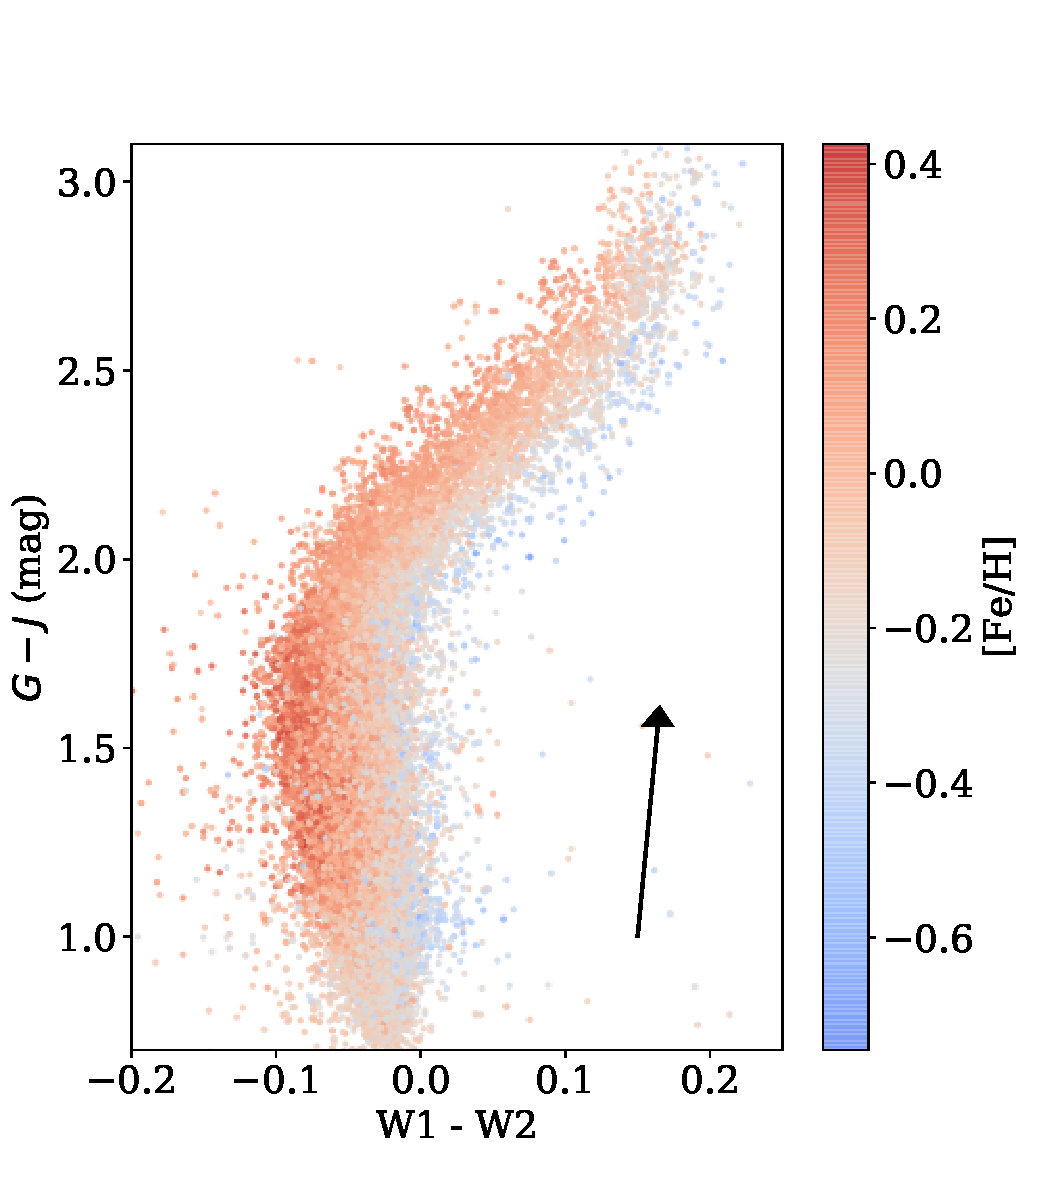
\includegraphics[height=2.5in]{color_color}
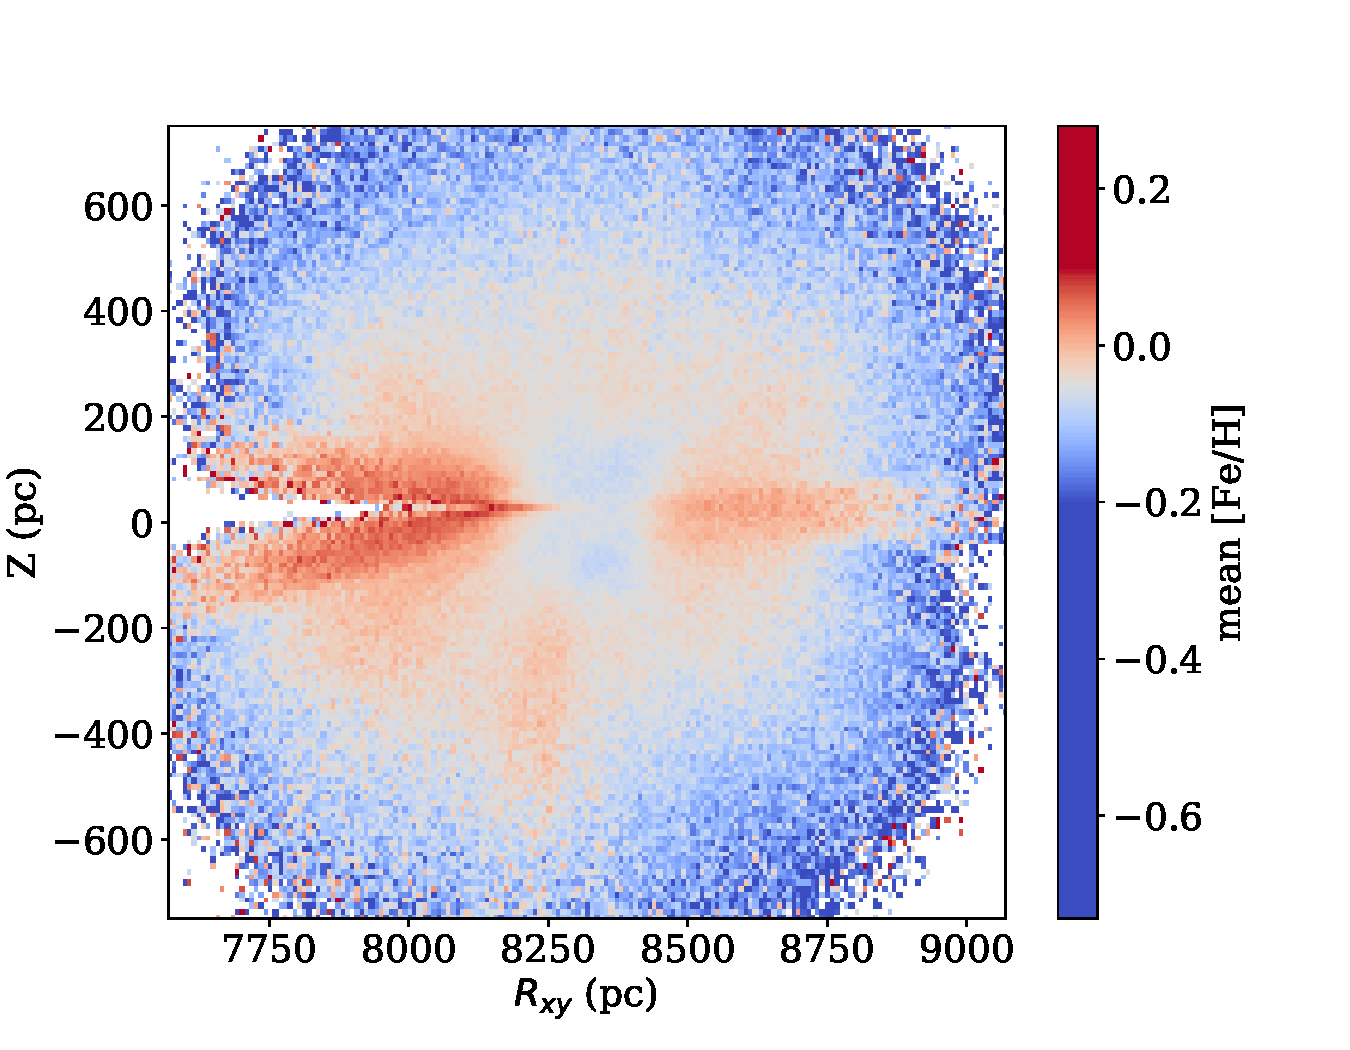
\includegraphics[height=2.5in]{RZ1}
\caption{
Left: Color--color training diagram for the 35,210 APOGEE stars colored by their measured metallicities. This sample is used to train our {\tt KNN} algorithm \ingot. A reddening vector from \citet{sanders18} for 1 mag of $V$-band extinction is shown for reference.
Right: Average metallicity in our 3 million star ALLWISE-Gaia sample projected on cylindrical  ($R_{xy}$, Z) coordinates. The metal-rich Galactic disk is clearly seen. The apparent break in the disk near the solar position is due to sample incompleteness of high proper-motion objects.
\label{fig:1}}
\end{figure*}

Following Figure 5 of \citet{schmidt16}, we trained \ingot on \feh as a function of ($W1-W2$, $G-J$), shown in Figure \ref{fig:1}. We used 35,210 stars from the APOGEE Stellar Parameters and Chemical Abundances Pipeline \citep[ASCAP,][]{garcia-perez2016}, cross-matched to ALLWISE \citep{mainzer2014} and Gaia DR2 using the CDS X-Match service with a 1 arcsec search radius. The $J$-band magnitude comes from 2MASS \citep{2mass}, and is pre-matched to WISE. $G-J$ (Gaia - 2MASS) spans a wide wavelength range, and is a good proxy for stellar effective temperature. As \citet{schmidt16} note, $W1-W2$ shows a small amplitude gradient that correlates with \feh ($\sim$1 dex in \feh over $\sim$0.1 mag in color).


To represent our data with a flexible model, we used {\tt scikit-learn}'s {\it k}-nearest neighbors (KNN) regression, with the default neighbor distance of $k=5$. This model can rapidly estimate \feh values for any new star given ($W1-W2$, $G-J$), and be easily recomputed given additional axes including the absolute Gaia magnitude ($M_G$). Crude uncertainties can be computed by examining the standard deviation of the measured versus predicted \feh values, which found typical scatter of $\sigma\approx0.11$ dex in our training sample. This does not account for photometric errors, nor correct for extinction in any of the bands.


We applied \ingot to 3.8 million new low-mass stars selected from Gaia and WISE photometry for stars within the color--color box defined in Figure \ref{fig:1}, reaching $\sim$600 pc over the entire sky. The mean \feh for these sources projected into the ($R_{xy}, Z$) plane is shown in Figure \ref{fig:1}. The metal-rich disk of the Milky Way, including the decreasing scale-height with increasing radius, is clearly recovered.


\ingot is publicly available\footnote{https://github.com/jradavenport/ingot}, including the data required to recreate our training sample. We consider \ingot a demonstration of the  potential for simple machine learning tools combined with multi-wavelength data from wide-field surveys to advance galactic chemical cartography. For example, the catalog of over 2 billion point sources from the unWISE project \citep{schlafly2019}, matched to Gaia DR2, is an ideal dataset for such analysis.




%%%%%%%%%
\acknowledgments

This work has made use of data from the European Space Agency (ESA) mission
{\it Gaia} (\url{https://www.cosmos.esa.int/gaia}), processed by the {\it Gaia}
Data Processing and Analysis Consortium (DPAC,
\url{https://www.cosmos.esa.int/web/gaia/dpac/consortium}). Funding for the DPAC
has been provided by national institutions, in particular the institutions
participating in the {\it Gaia} Multilateral Agreement.

This publication makes use of data products from the Near-Earth Object Wide-field Infrared Survey Explorer (NEOWISE), which is a project of the Jet Propulsion Laboratory/California Institute of Technology. NEOWISE is funded by the National Aeronautics and Space Administration.

\software{Python, IPython \citep{ipython}, NumPy \citep{numpy}, Matplotlib \citep{matplotlib}, SciPy \citep{scipy}, Pandas \citep{pandas}, Astropy \citep{astropy}, Scikit-Learn \citep{scikit-learn}}


\bibliography{bib}


\end{document}
